\documentclass[10pt, hyperref={unicode}]{beamer}
\usepackage[czech]{babel}
\usepackage[utf8]{inputenc}
\usepackage{times} % font
\usepackage{listings} % algoritmy
\usepackage{graphics} % vkládání obrázků
\graphicspath{array.png}


\usetheme{Singapore}
\setbeamertemplate{footline}[frame number]
\setbeamertemplate{frametitle}[default][center]

\lstdefinestyle{CustomStyle}{
  language=C,
  numbers=left,
  showspaces=false,
  showstringspaces=false,
  frame=single,
  keepspaces=true
}

\title{Typografie a publikování -- 5. projekt}
\subtitle{Datové struktury -- Pole}
\author{Maxim Plička}
\date{\today}
\institute
{
	Vysoké učení technické v Brně\\
	Fakulta informačních technologií
}
\begin{document}
\maketitle

\begin{frame}{Přehled}
\begin{itemize}
    \item Proč jsem si vybral pole?
    \item Definice
    \item Operace nad polem
    \item Ukázky operací
    \item Konec
\end{itemize}
\end{frame}

\begin{frame}{Proč jsem si vybral pole?}
\begin{itemize}
    \item Jednoduchost používání
    \item Rozšířenost
    \item Pozitivní zkušenost
\end{itemize}
\end{frame}

\begin{frame}{Definice}
\begin{itemize}
    \item Datová struktura, která je v paměti uložena jako posloupnost prvků stejného typu.
    \item K jednotlivým hodnotám přistupujeme pomocí indexu).
    \item Každý prvek má svůj vlastní index (indexuje se od nuly).
    \item Podle velikosti se dělí na: 
    \begin{itemize}
          \item Jednorozměrne pole
          \item Dvourozměrné pole
          \item N-rozměrné pole
    \end{itemize}
    \begin{figure}[t]
    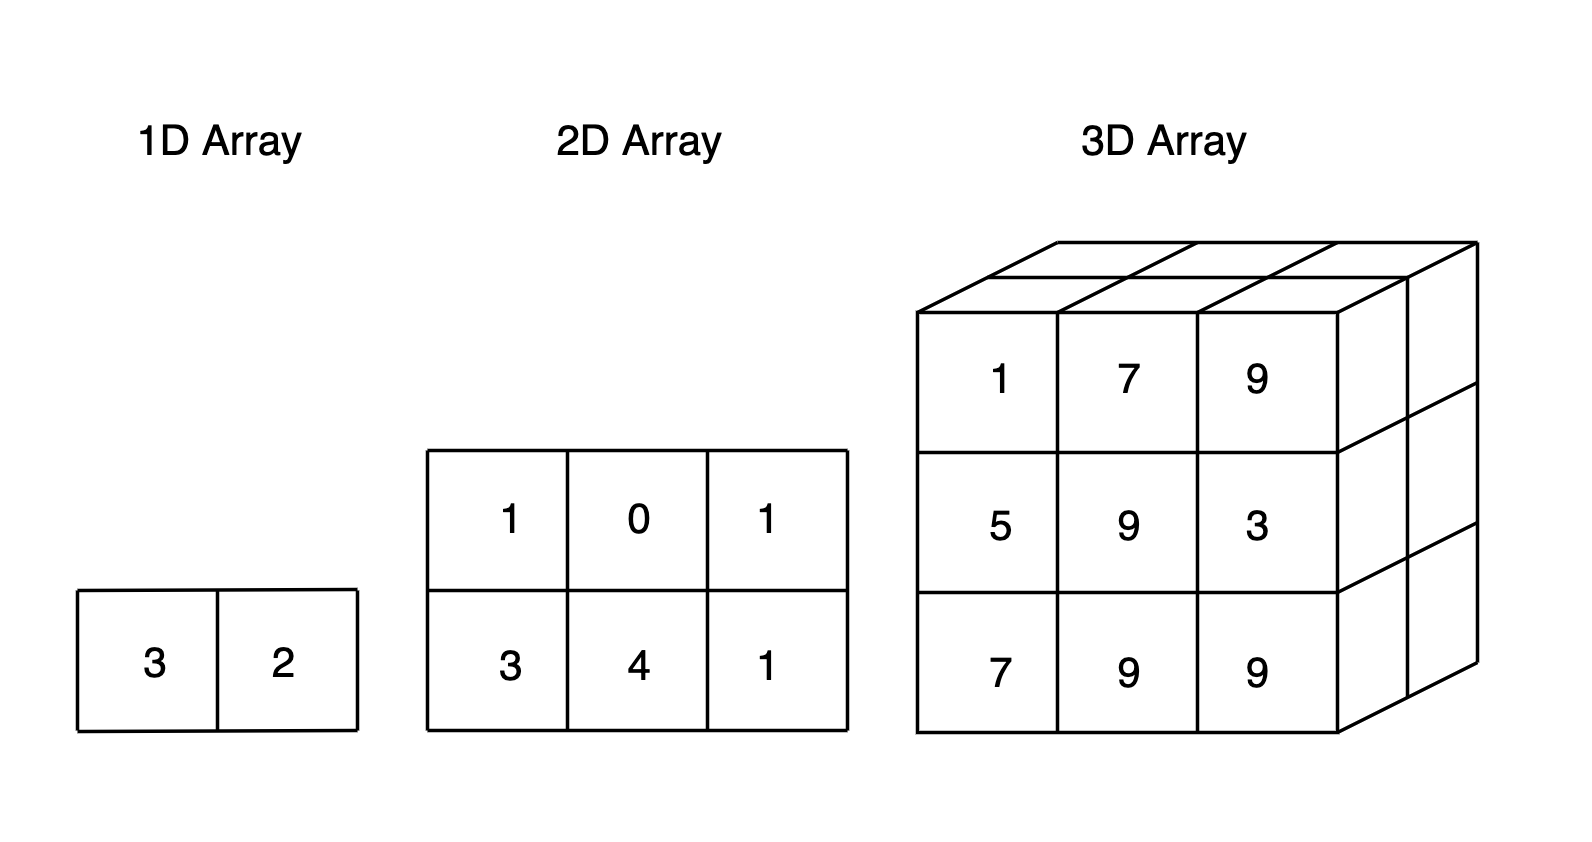
\includegraphics[scale=0.12]{array.png}
    \end{figure}
\end{itemize}
\end{frame}

\begin{frame}{Operace nad polem}
\begin{itemize}
    \item Přístup k prvku 
        \begin{itemize}
        \item Přesnou adresu v paměti lze získat pomocí indexu (pointerová aritmetika)
        \end{itemize}
    \item Vyhledávání prvku v seřazeném poli 
        \begin{itemize} 
        \item využívá \alert{metodu půlení intervalů} indexů pole
        \end{itemize}
    \item Vyhledávání prvku v neseřazeném poli
        \begin{itemize}
        \item Lineární průběh
        \item V nejhorším případě je nutné projít celé pole
        \end{itemize}
\end{itemize}
\end{frame}

\lstset{basicstyle=\small,style=CustomStyle}
\begin{frame}[fragile]{Ukázka 1/2}
Inicializace pole čísel o velikosti i.
\begin{lstlisting}
int array[i];
\end{lstlisting}
Přiřazení hodnoty 2 do posleního prvku pole.
\begin{lstlisting}
int array[i-1] = 2;
\end{lstlisting}
\end{frame}

\begin{frame}[fragile]{Ukázka 2/2}
Listování v poli o velikosti N$\times$M prvků + výpis hodnot.
\begin{lstlisting}
int array[n][m];
for(int i = 0; i < n; i++)
{
    for(int j = 0; j < m; j++)
    {
        printf("%d",array[n][m]);
    }
}
\end{lstlisting}
\end{frame}

\begin{frame}{Konec}
\begin{itemize}
    \item Díky za pozornost
\end{itemize}
\end{frame}

\end{document}